\subsubsection{Delete and shift}
After $B$ extracts the public key of $C$, it deletes the routing information from the packet. $B$ then fills the empty space with its own blinding (which is different from the one received from $A$) by setting the key share $\alpha_0$ to $\alpha_1=g^{xb_0}$. $B$ also computes $\beta_1$ as follows:

The first $\kappa$ bits of $\beta_0$ will be $n_{1}$ itself, the next $\kappa$ bits will be $\gamma_{1}$, and the remaining $(2r-1)\kappa$ bits of $\beta_0$ are shifted left to form the leftmost $(2r-1)\kappa$ bits of $\beta_{1}$; the rightmost $2\kappa$ bits of $\beta_{1}$ are simply a substring of an output of the PRG function.

\begin{figure}[H]
    \centering
    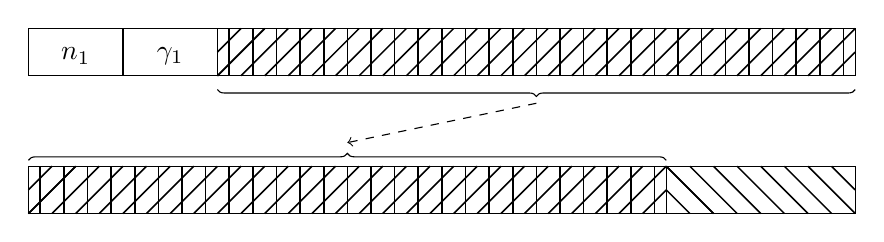
\begin{tikzpicture}
        \def\betaLength{10.5}
        \def\pubKey{1.2}
        \def\authTag{1.2}
        \draw (0,0) rectangle (\betaLength,0.6);

        \draw (0.6, 0.25) node {$n_1$};
        \draw (1.8, 0.25) node {$\gamma_1$};

        \draw (\pubKey,0) -- (\pubKey,0.6) (\pubKey+\authTag,0) -- (\pubKey+\authTag,0.6);

        \draw[decoration={brace,raise=5pt,mirror},decorate] (\authTag+\pubKey,0) -- (\betaLength,0);

        \def\halfBeta{{(\betaLength-\pubKey-\authTag)}*0.5}
        \draw [->,dashed] (4.05+\pubKey+\authTag, -0.35) -- (4.05, -0.85);

        \draw[decoration={brace,raise=5pt},decorate] (0,-1.25) -- (\betaLength-\authTag-\pubKey,-1.25);

        \begin{scope}[shift={(\pubKey+\authTag,0)}]
            \def\a{8.1}
            \def\b{0.6}
            \def\lw{0.2}
            \def\diff{7.5}

            \foreach \x [count=\i] in{0,0.3,0.6,...,\b}{
                    \draw [line width=\lw mm](0,\x)--(\b-\x,\b) (\a-\b+\x,0)--(\a,\b-\x);
                }
            \foreach \x [count=\i] in{0,0.3,0.6,...,\diff}{
                    \draw [line width=\lw mm](\x,0)--(\b+\x,\b);
                }

            \foreach \x [count=\i] in{0,0.15,0.45,...,\a}{
                    \draw [line width=\lw mm](\x,0)--(\x,\b);
                }
        \end{scope}

        \begin{scope}[shift={(0, -1.75)}]
            \draw (0,0) rectangle (\betaLength,0.6);
            \draw (\betaLength-\pubKey-\authTag, 0) -- (\betaLength-\pubKey-\authTag, 0.6);

            \begin{scope}[shift={(0,0)}]
                \def\a{8.1}
                \def\b{0.6}
                \def\lw{0.2}
                \def\diff{7.5}

                \foreach \x [count=\i] in{0,0.3,0.6,...,\b}{
                        \draw [line width=\lw mm](0,\x)--(\b-\x,\b) (\a-\b+\x,0)--(\a,\b-\x);
                    }
                \foreach \x [count=\i] in{0,0.3,0.6,...,\diff}{
                        \draw [line width=\lw mm](\x,0)--(\b+\x,\b);
                    }

                \foreach \x [count=\i] in{0,0.15,0.45,...,\a}{
                        \draw [line width=\lw mm](\x,0)--(\x,\b);
                    }
            \end{scope}

            \begin{scope}[shift={(\betaLength-\pubKey-\authTag,0)}]
                \def\a{2.4}
                \def\b{0.6}
                \def\lw{0.2}
                \def\diff{1.8}
                \foreach \x [count=\i] in{0,0.3,0.6,...,\b}{
                        \draw [line width=\lw mm](\x,0)--(0,\x) (\a-\b+\x,\b)--(\a,\x);
                    }
                \foreach \x [count=\i] in{0,0.3,0.6,...,\diff}{
                        \draw [line width=\lw mm](\x+\b,0)--(\x,\b);
                    }
            \end{scope}
        \end{scope}

    \end{tikzpicture}
    \caption{Shifting in the header}
\end{figure}

The new mix header is now ready to be sent to $C$, defined as the node with public key $y_1$:

$$M_1=(\alpha_1,\beta_1,\gamma_1)$$

where $\alpha$, $\beta$ and $\gamma$ are defined in equations $\ref{eq:1}$, $\ref{eq:2}$ and $\ref{eq:6}$